\chapter[Remote shell]{Le remote shell}
Retour au remote shell. Comme il avait été testé, le processus ssh ne prend pas ce qu'on lui envoie depuis la file car ce n'est pas un terminal. La question étant : qu'est-ce qu'il concerne comme un terminal ? Si le programme crée un processus bash qui crée le ssh, est-ce que cela lui irait ? Testons cela.
\\\\
Oh, juste avant de le tester, j'ai ajouté au programme une option, utilisable via "-v" ou "--verbose". Si elle est activée, le programme affiche l'arbre syntaxique avant d'exécuter la commande. Rien d'incroyable.
\\\\
Bon, je sais, je temporise beaucoup, mais je viens d'effectuer des tests pour le mode verbeux, et j'en ai profité pour lancer notre programme dans notre programme. Aucun souci. Mais je me dis que si le remote shell fonctionne (si on y arrive), on nous demandera probablement d'exécuter "remote all ./Termina". Et ça doit fonctionner. Je m'inquiète un peu pour cette fonctionnalité.
\\\\
Je viens de regarder le scipt shell xcat.sh. Constat : il y a la commande mkfifo. Maintenant, ne serait-il pas plus simple d'ouvrir des fenêtres, et de s'en servir comme entrée / sortie de nos connexions ssh ? Et que le tout reste contrôlable via notre terminal principal ?
\\\\
AH ! J'AI OUBLIÉ LES PROCESSUS ZOMBIES ! Shit. Bon tant pis, ce sera pas fait. Il fallait juste créer uns structure de données du genre liste chaînée ou tableau extensible, et enregistrer les pids à chaque fork. Dès qu'un wait avait fini, on retirait le pid de la liste. En fin de programme (exit, éventuellement intercepter quelques signaux), on parcours la liste et on les tue tous à grand coup de "kill -9".
\\\\
J'essaie, actuellement, de simplement lancer un fils ssh. Aucun affichage ne se fait sur stdout. J'ai bien peur que ssh n'accepte réellement que les terminaux en entrée. Je fais quelques recherches sur le net, mais ça n'a vraiment pas l'air simple. Il semblerait que ce soit cette seule phase d'authentification qui bloque tout. La suite n'a pas l'air difficile, ça n'a l'air d'être que de l'écriture dans un pipe.
\\Histoire de suivre mes recherches, je vais lister toutes les solutions que je vois passer, sans qu'elles soient forcément adaptées (certaines n'ont même rien à voir). J'ai aussi demandé à certains ce qu'ils avaient fait, sans détailler. Deux réponses : "ssh <serveur> bash", et "libssh". Le premier, ça ne laisse pas passer l'authentification et mess-up avec les entrées / sorties, et le second, c'est hors de question d'utiliser une bibliothèque, c'est un choix trop facile. Bref, voilà la liste :
\begin{itemize}
\item screen
\item nohup
\item disown
\item xterm/gnome-terminal
\item Cluster SSH
\item PAC Manager
\item OpenSSH
\\\end{itemize}
Tiens, un tutoriel pour le faire en Python\footnote{\url{https://amoffat.github.io/sh/tutorials/2-interacting_with_processes.html}}. Et devinez la première phrase : "Using subprocesses to interact with SSH is notoriously difficult". No kidding. "It is recommended that you just ssh-copy-id to copy your public key to the server so you don’t need to enter your password, but for the purposes of this demonstration, we try to enter a password".
\\J'ai donc la confirmation que je voulais. Ce projet demande sûrement de se connecter à des serveurs sans authentification. Cependant... Cependant je ne me réduirai pas à ça. Cette commande est juste incroyable. Si on parvient à la mettre en place sous cette forme, c'est beaucoup mieux. Contrôler pleinement depuis un seul terminal plusieurs connexions ssh. Certes, je désobéis au sujet, mais "remote" n'a plus aucun intérêt si on zappe l'authentification. Le projet ne sera probablement pas terminé, car il me reste peu de temps, mais je veux rester là-dessus.
\\\\
Je lis donc le tutoriel que j'ai mentionné plus tôt. Et il parle de buffering ! Le problème n'est pas que l'entrée n'est pas un terminal, mais que le buffer contient un '\textbackslash{n}'. En changeant la méthode de bufferisation, on peut régler ce problème. Dans le sujet, ils mentionnent fdopen() et setvbuf() pour cet effet. J'ai trouvé des exemples d'utilisation, mais pas sur des pipes. J'ai du mal à comprendre la façon de l'utiliser. Je crée un seul fichier FILE* que je bufferise, et les deux processus lisent / écrivent dedans (une sorte de faux pipe), ou je dois créer mon pipe, créer les FILE* correspondant aux deux extrémités, et les bufferiser ? C'est simple : aucun des deux ne fonctionne. Je ne peux pas rediriger des entrées sorties dans des flux, dup() ne fonctionne qu'avec des descripteurs de fichiers.
\\La solution privilégiée par le tutoriel, c'est de ssh-copy-id avant tout. Pour notre programme, ça voudrait dire que si la connexion ne se fait pas, on demande à l'utilisateur de lancer ssh-copy-id en premier. On revient à la connexion sans identification. Juste pour une histoire de bufferisation.
\\\\
J'y vais progressivement. J'ai trouvé la réponse à ma question. Le côté lecture du pipe, on s'en fiche. C'est l'écriture qu'on prend comme stream. En faisant ça, on décide quand est-ce que le pipe reçoit de l'information. Je dois maintenant utiliser fputs() pour écrire dans mon stream / pipe. Ça fonctionne assez bizarrement tout de même, mais ça m'arrange. Si je dois envoyer la commande au ssh, je crois l'envoyer d'un bloc. Je suppose. Donc je dois faire plusieurs fputs(). Mais après un test (afficher une chaîne spéciale après l'affichage du buffer par le fils), plusieurs fputs() à la suite ne déclenchent pas de flush du stream. Ce qui est parfait pour envoyer la commande mot par mot, et ajouter les espaces, sans batailler.
\\Hum. Ce n'est pas parfait. L'ajout des espaces semble créer un décalage de bits. Des caractères étranges s'affichent.
\begin{figure}[!htp]
\centering
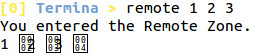
\includegraphics[width=200pt]{Axel-06_RemoteChars.jpg}
\end{figure}
\\Je ne sais trop peu quoi en penser. Je tente quelque chose... Et ça fonctionne. Je passais un caractère espace par référence, et ça déconnait, alors qu'en l'écrivant en dur dans fputs (je ne savais pas qu'on pouvait... c'était logique pourtant), ça passe sans souci.
\\Bien ! On arrive a envoyer des donnés via un buffer. Maintenant, il faut tester d'envoyer un mot de passe à une connexion ssh via ce buffer, et tester différentes bufferisations. Pour l'instant, ssh affiche bien sur le terminal, et demande le mot de passe. Problème : je ne peux pas le valider. Là, j'étais en \_IONBF (sans bufferisation. Tentons par ligne, \_IOLBF. Pas mieux. Et en bufferisation totale, \_IOFBF ? Toujours pas. Je pensais que bufferisé par ligne fonctionnerait. Et si je tente d'afficher quelque chose une fois que le père a fini ? AAAAHHHH, JE NE COMPRENDS RIEN ! Avec fwrite(), c'est le même délire. Je ne comprends pas. Le comportement change. Selon quand j'appuie sur Enter, le programme ne fait pas la même chose. Des fois, il est ajouté au buffer, parfois affiché, parfois on passe au read() suivant. Sans bufferisaton, je comprends mieux. Enter provoque un flush à chaque fois.
\\\\
J'ai possiblement un indice sur le problème. J'ai essayé de ne pas m'occuper du fils, et de tout simplement afficher le buffer une fois lu, et envoyé dans le stream. Il est lu, et bien affiché. Le père boucle à l'infini dans le while(read). Rien de surprenant. La sortie, que ce soit du père ou du fils, est conforme à l'entrée, incluant le '\textbackslash{n}'. Ça ne vient pas de la communication, mais encore du ssh... Quel bordel.
\\\\
Ok. C'est bon. Je suis vaincu. J'abandonne. J'y arrive pas. Ça fait plusieurs heures que je suis dessus, et aucune avancée. J'en peux plus. Je n'ai jamais autant eu cette impression d'échec. Je n'avance sur rien.